\chapter{The LHC and the ATLAS detector}
\section{The LHC}

Due to the statistical nature of Particle Physics it does not only require sufficiently high energies but also an exceedingly large amount of data to allow significant results.
The LHC provides both with an energy of and an integrated luminosity of.
The analysis in this work used data(?) based on the ATLAS detector, on of the four detectors at the LHC.

This chapter introduces the LHC, followed by the most important aspects of the ATLAS detector. In the next ch

\section{The ATLAS detector}

\subsection{Tracking Detectors}

\subsection{Calorimeter (split)}

\subsection{Muon Spectrometer}

\subsection{How the detector works}

\subsection{The LHC}

The Large Hadron Collider ("LHC") located at the facilities of the European Organization of Nuclear Research ("CERN") close to Geneva was built to extend the frontiers of modern particle physics by delivering high luminosities and reaching unprecedented high energies.
The LHC is designed to collide bunches of up to \num{d11} protons at a luminosity of \SI{d34}{\per\square\cm \per\s}. The beams collide at four points where the four main experiments of the LHC are located. Two of these are special-purpose detectors, namely LHCb and ALICE while the other two, ATLAS and CMS, are general-purpose detectors.
This experiment uses ATLAS data and Monte Carlo.
Figure \ref{fig:LHC} shows the LHC, the four detectors and its general location.
\begin{figure}
  \centering
  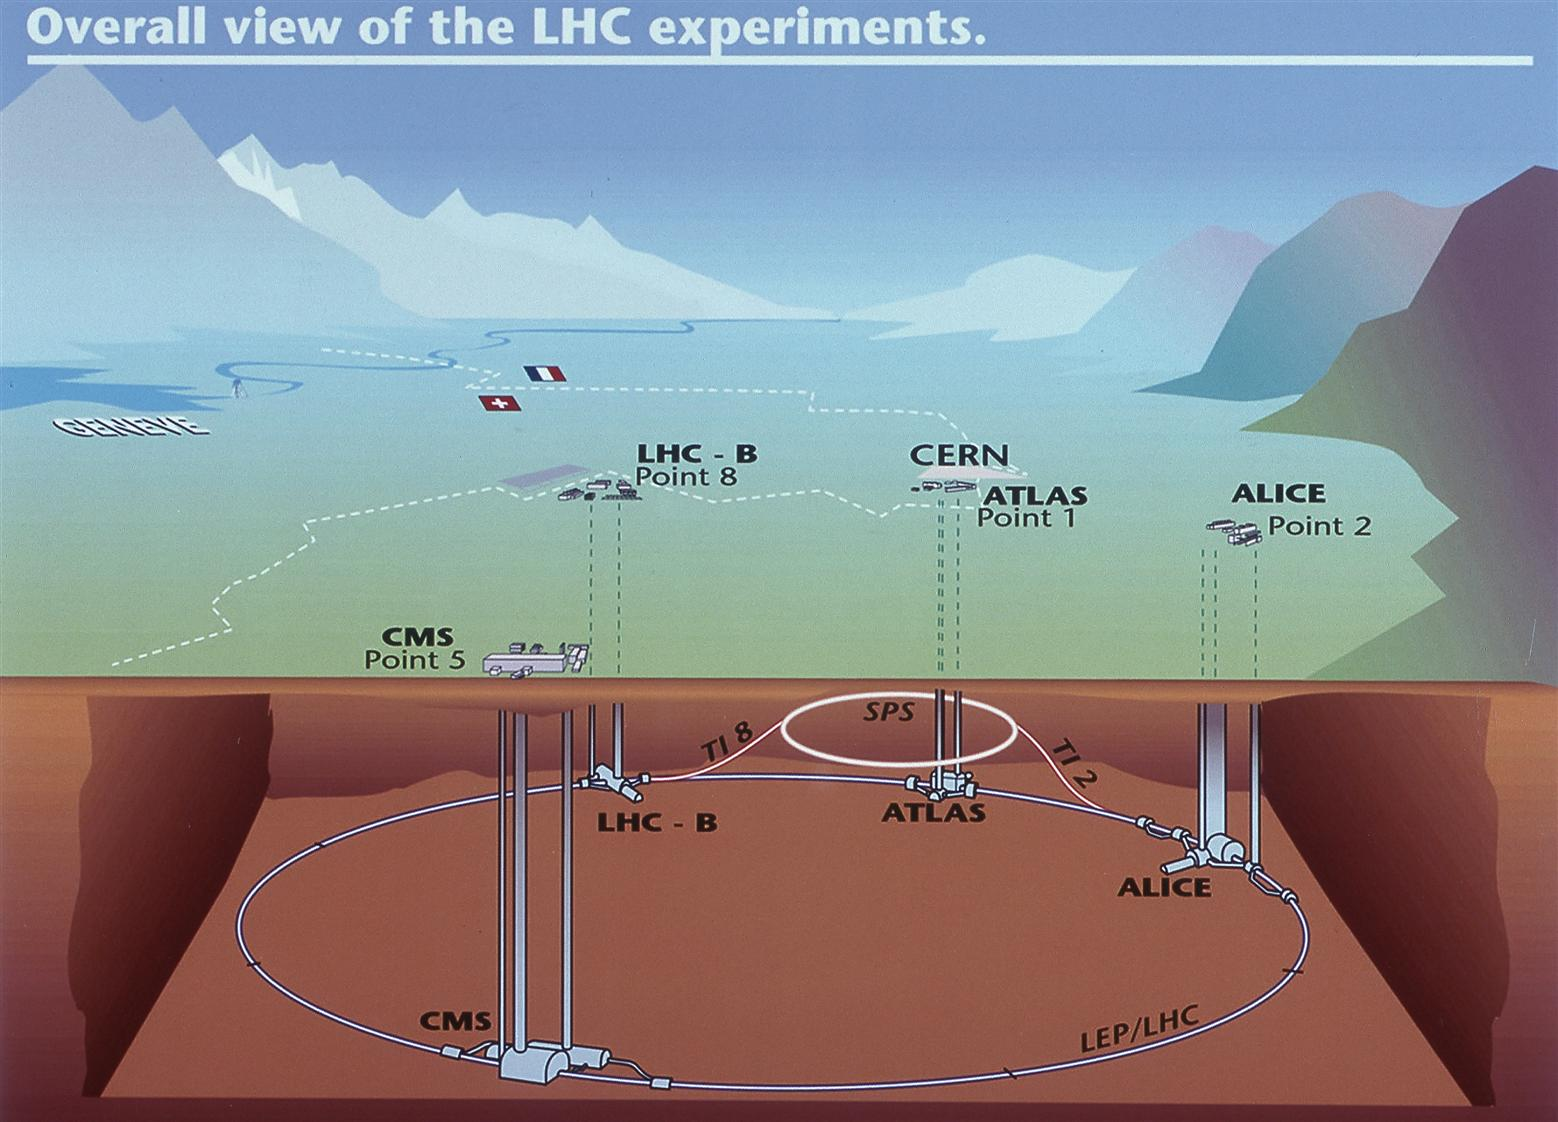
\includegraphics[scale=0.4]{figures_LHC/CERN-all-experiments.jpg}
  \caption[Sketch of the LHC ring.]{Sketch of the LHC ring, the position
    of the experiments and the surrounding countryside. The four big
    LHC experiments are indicated(ATLAS, CMS, LHC-B and ALICE)along with their injection lines(Point 1, 2, 4, 8)\cite{atlas_pictures}}
  \label{fig:LHC}
\end{figure}


\subsection{The ATLAS Detector}

The ATLAS detector was developed to study the physic processes in a broad energy range available at the LHC. This enables the observation of highly massive particles that lower energy accelerators were not able to create and that would deliver new physics theory beyond the standard model of particle physics.
It was designed to cover the maximum number of final states being a so called general purpose-detector.

\begin{figure}
  \centering
  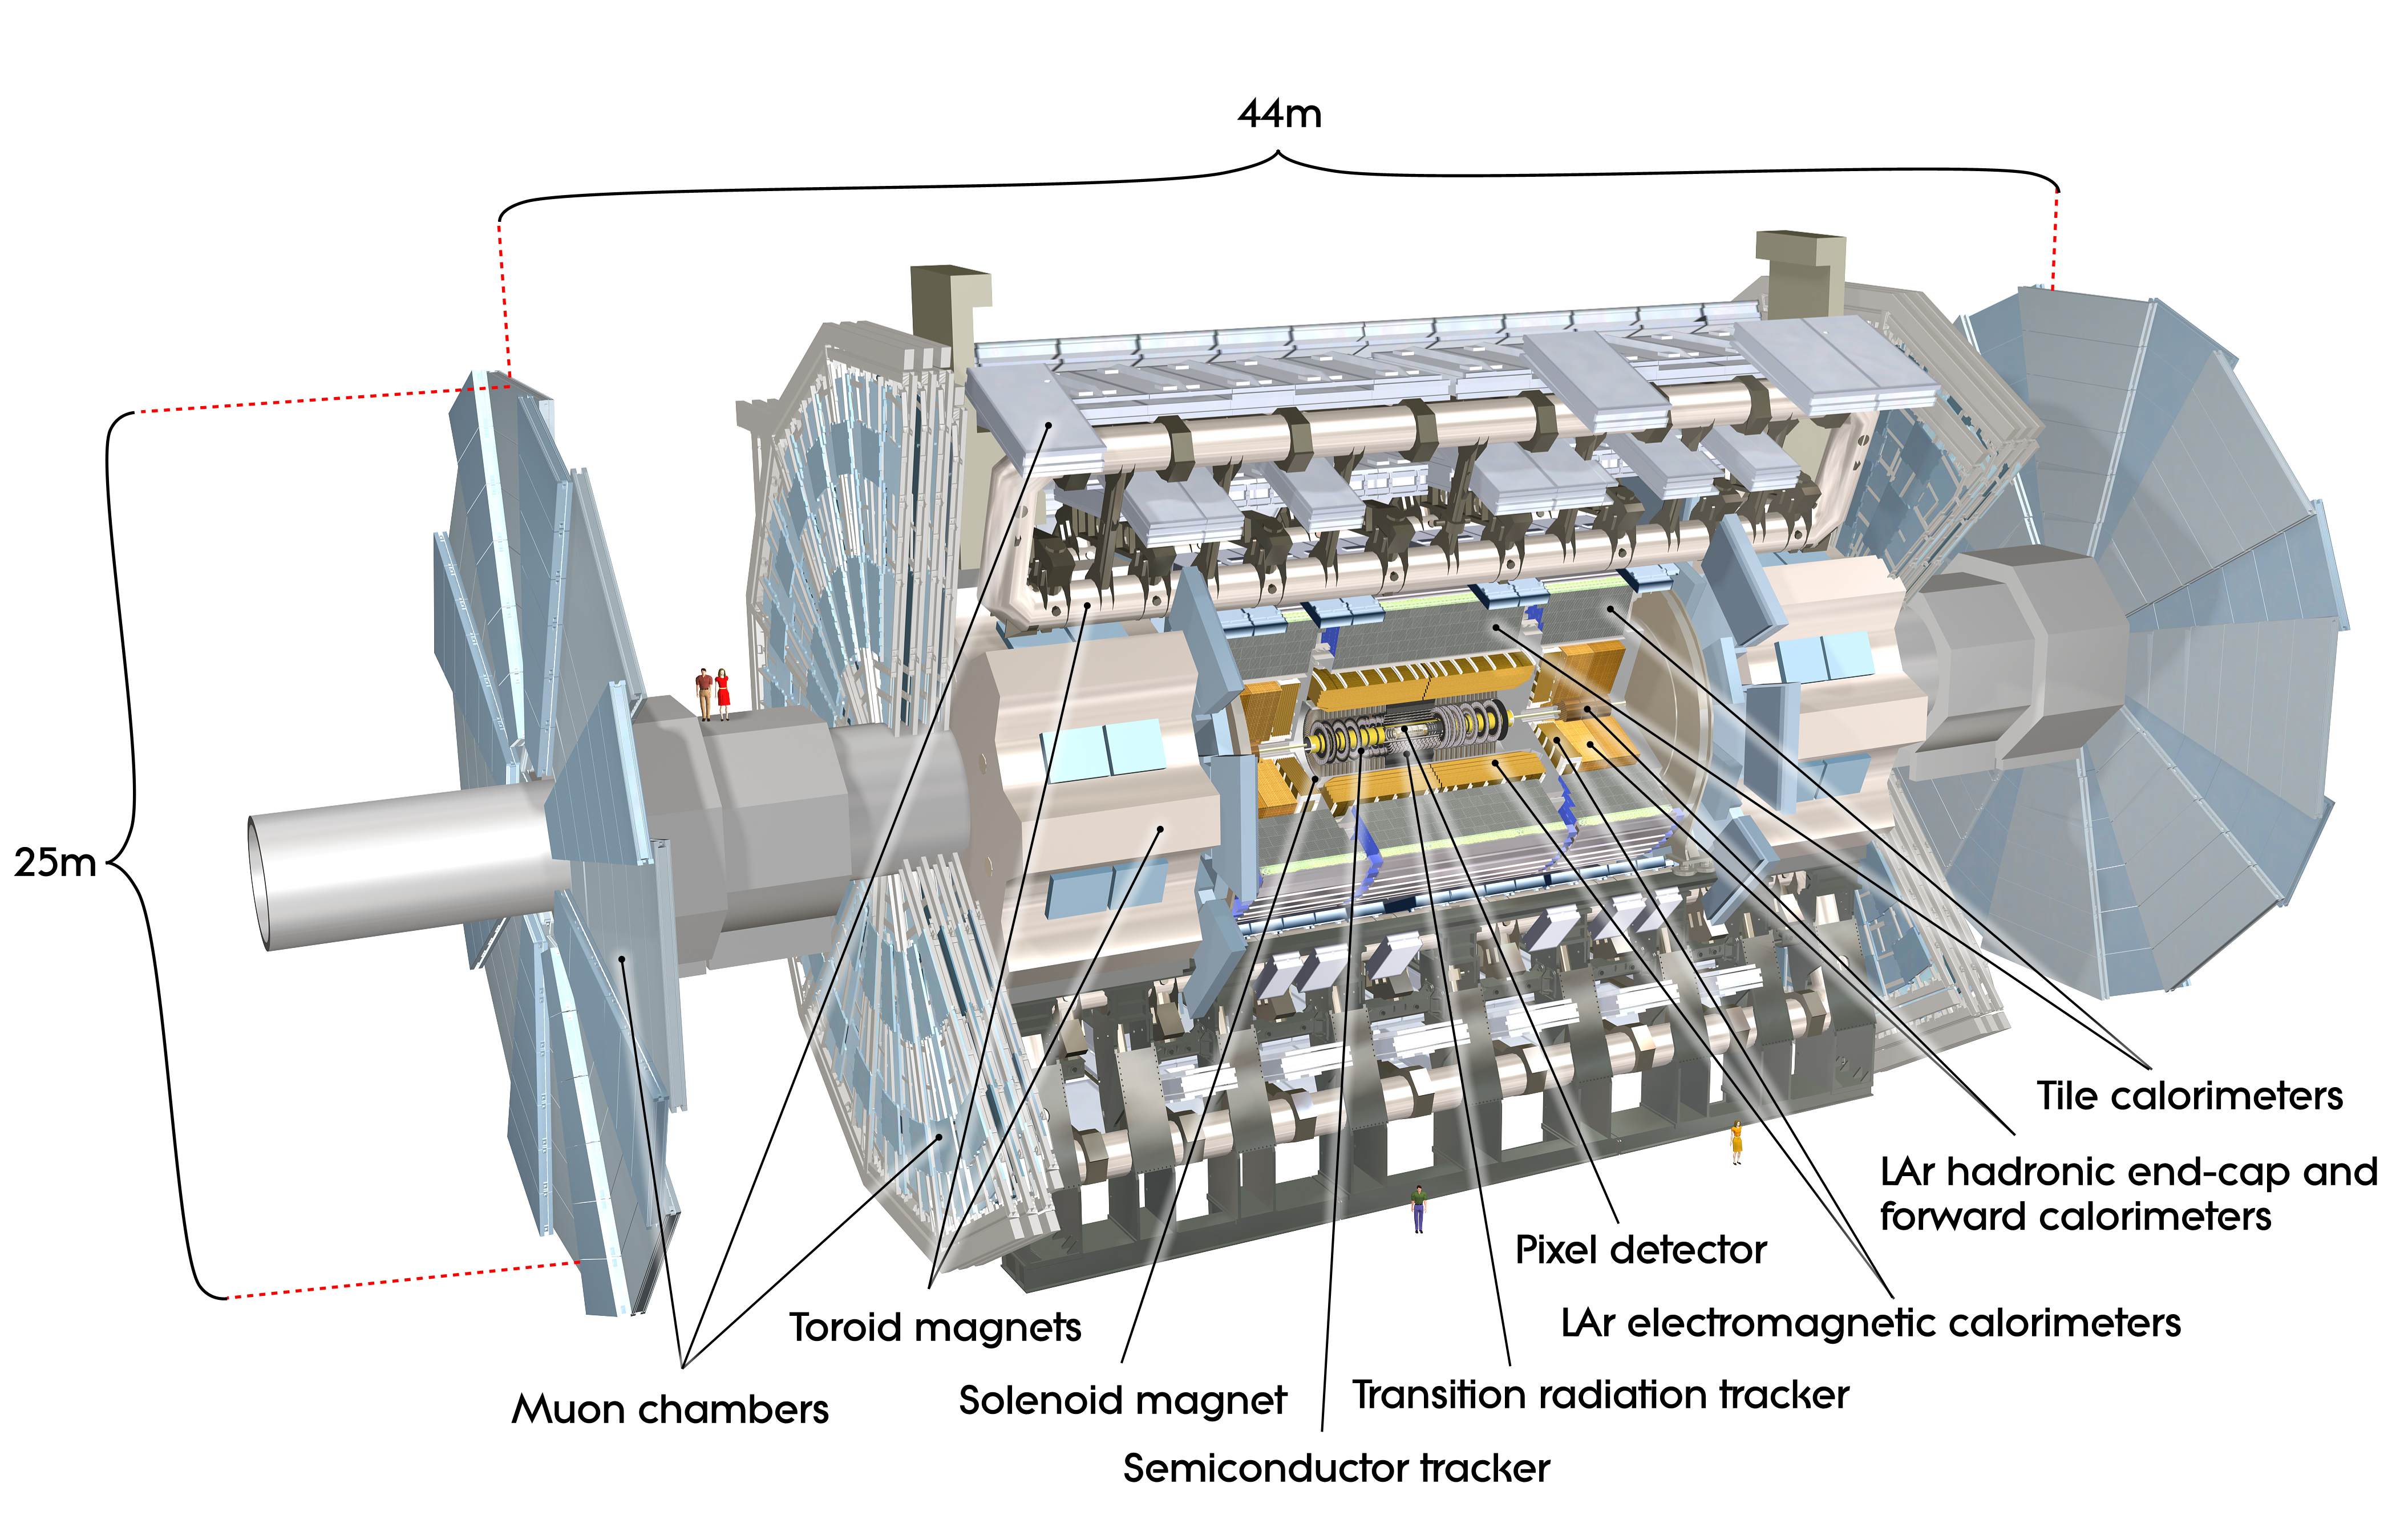
\includegraphics[scale=0.15]{figures_LHC/atlas-detector}
  \caption{Sketch of the ATLAS detector}
  \label{fig:atlas}
\end{figure}



\begin{figure}
  \centering
  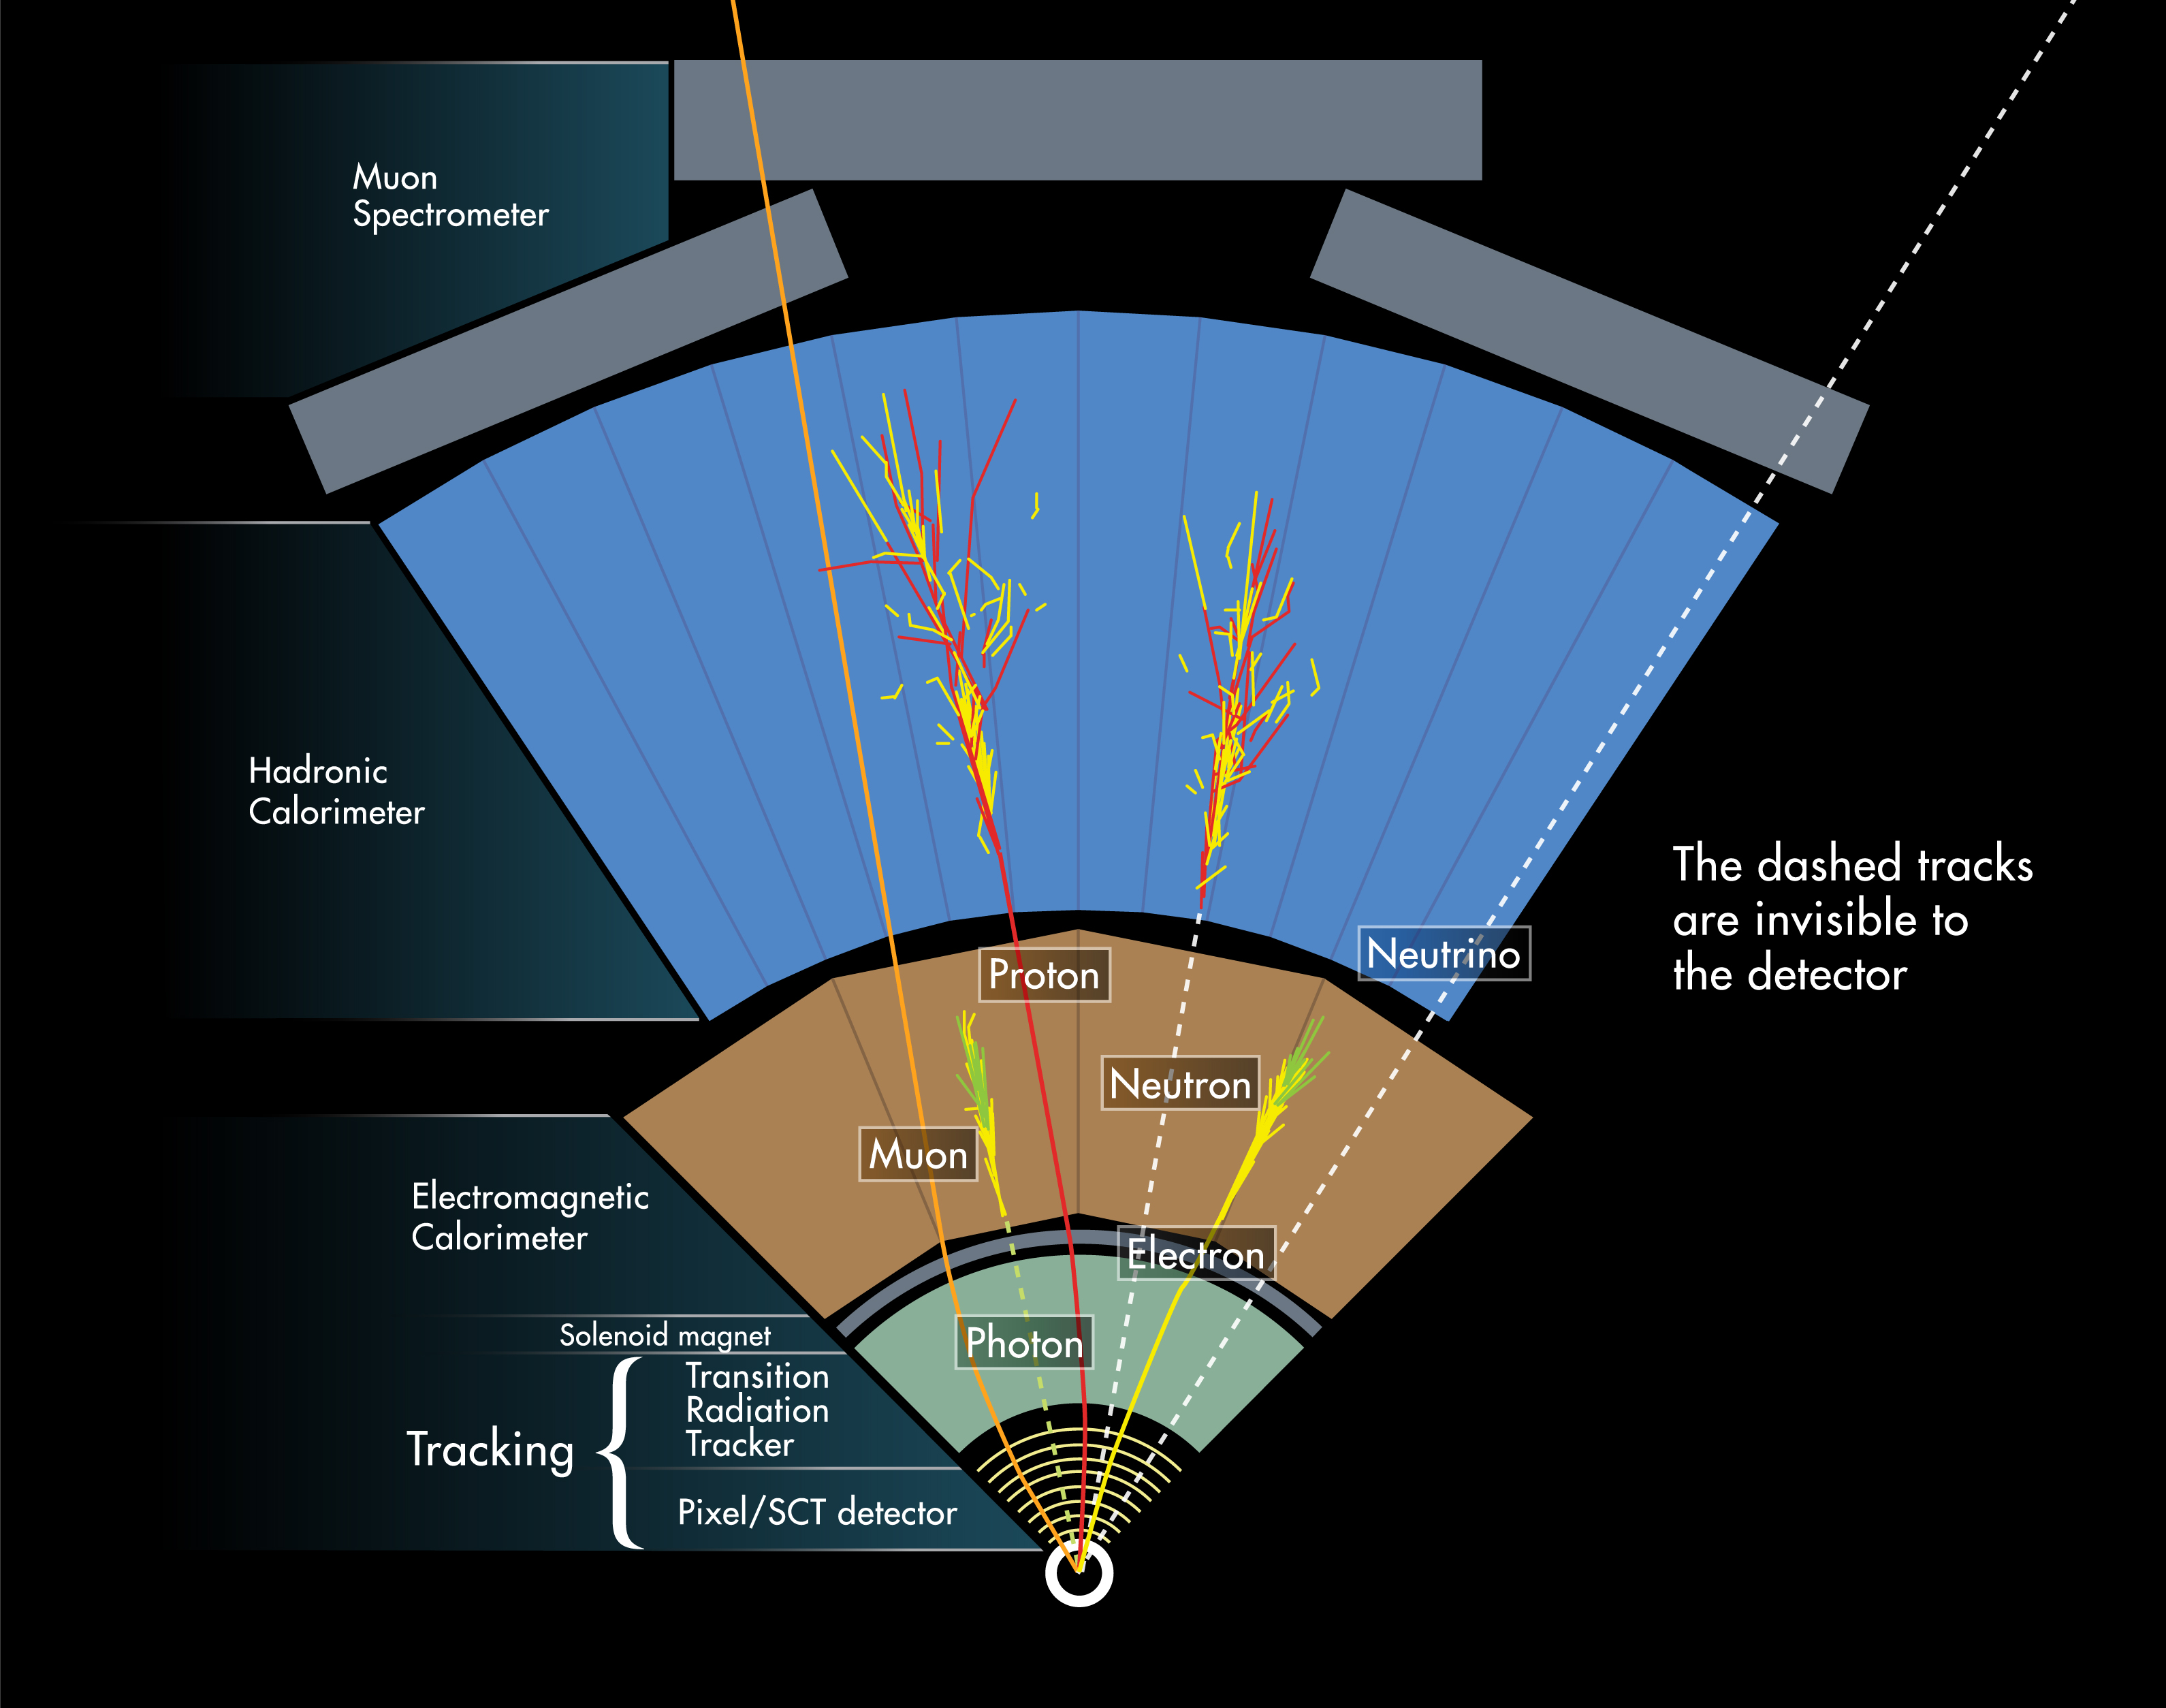
\includegraphics[scale=0.6]{figures_LHC/atlas-abstract}
  \caption[Scheme of the ATLAS-detector.]{Scheme of the ATLAS-detector with examples of tyical particle detections. \cite{atlas_pictures}}
  \label{fig:atlas_sketch}
\end{figure}

\subsection{The ATLAS coordinate system}

The ATLAS coordinate system is defined by the beam direction with the $z$-axis pointing along the LHC's beam pipe. The corresponding transverse plane is defined by the $x$-axis pointing towards the ring's centre while the $y$-axis points upwards. The origin of the system is defined by the nominal point of interaction. The polar angle $\theta$, is the angle between the $z$-axis and the $x$-$y$-plane and the azimuthal angle $\phi$ is the angle between the $x$- and the $y$-axis.

The coordinates used in this analysis are usually the azimuthal angle $\phi$, the pseudo-rapidity $\eta$, and the transverse momentum $pT$. The pseudo-rapidity replaces the polar angle and is defined as

\begin{equation}
\eta = \frac{1}{2} ln\left[ tan\left(\frac{\theta}{2}\right)\right].
\end{equation}

The transverse momentum is defined by

\begin{equation}
pT = \sqrt{p_x^2 + p_y^2}
\end{equation}
where $p_x$ and $p_y$ are the momenta along the corresponding axes. 

The angular variables are defined within

\begin{equation}
\eta \in [-\infty,\infty],\,
\phi \in [-\pi,\pi].
\end{equation}
\subsection{Tracking detectors}

To measure momentum, trajectory and charge of charged particles usually tracking detectors are used.

There are two main categories of tracking detectors following the same general principle, gaseous detectors and semiconductor detectors. If ionizing radiation passes any given medium it will create electron-hole pairs. These charge carriers can then be collected by an electric field. Depending on the detector the signal caused by the charge carriers can be related to the coordinate of ionization in space and time.

\begin{itemize}
\item Gaseous detectors: Gaseous detectors are based on the greater mobility of ions and electrons in the gas. The basis of the detector is usually a chamber filled with a proper gas. The gas contains an area of wires to which a strong electric field is applied. If gas atoms get ionized the charge carriers (electrons and ions) will drift to the wires and create a detectable signal. The wires give a rough estimation of space which is normally improved by calculating the exact ionization location from the drift time.

\item Semiconductor detectors: Semiconductor detectors are as their name implies based on crystalline semiconductor material such as silicon and germanium. Their working principle is quite similar to that of gaseous detectors but the gas is exchanged by solid semiconducting material. In semiconducting material ionizing radiation will create electron-hole pairs instead of electron ion pairs that then can travel in a strong electric field to be detected. The big advantage of semiconductor detectors over gaseous detectors is that the energy required to create an electron-hole pair is about 10 times lower than the energy needed to ionize gas atoms. These detectors are commonly structured into wafers or pixels that allow a determination of the space.
\end{itemize}

Usually a magnetic field surrounds tracking detectors to bend the track and that way be able to compute the particles momentum and charge based on the curvature.\cite{leo}


In the ATLAS detector both the inner detector and the muon spectrometer are tracking detectors.

\subsubsection{The Inner Detector}

The innermost part of the ATLAS detector is called the Inner Detector, which consists of three sub-components, the Pixel detector (Pixel), the Semi-Conductor Tracker (SCT) and a Transition Radiation Tracker (TRT). Each of these sub-detectors is divided into the so called barrel part and two end-caps. The Inner Detector covers a region of $|\eta| < \num{2.5}$.

\subsubsection{The Muon spectrometer}

The second tracking detector of ATLAS is the muon spectrometer which is the outermost part of the detector. The task of the spectrometer is to detect charged particles transversing the calorimeter without being stopped or deploying their complete energy, and to do both trigger and tracking to measure their momentum. Due to these two tasks the spectrometer is bifid with the first part being the trigger chamber covering a range of $|\eta|<2.4$, followed by the high-precision chamber with a range of $|\eta|<2.7$. The main detector's support feet cause a further gap at about $\phi = \ang{300}$ and $\phi = \ang{270}$.


\subsection{Calorimeters}

In particle physics a calorimeter is a device to measure first and foremost the total energy of a particle. Most of the time some positional information is taken  additionally.
The idea is that most particles loose all their momentum while crossing the calorimeter. Measuring the energy deposited this way gives a value for the particle's energy.
Usually a particle deposits its energy by initiating a particle shower, the energy of which is then collected and measured.
Calorimeters are distinguished by the main interaction of the particles one aims to detect. 

\subsubsection{Electromagnetic Calorimeters}

Electromagnetic calorimeters are designed to detect charged particles that primarily interact via the electromagnetic interaction and to measure their total energy. Usually these particles are electrons and photons. There are various methods to construct these detectors. An example would be the usage of inorganic scintillators. These scintillators should be optically transparent and have a short radiation length to contain the shower in a compact region. The detection can then be followed by photon detectors with photo-multipliers which measure the emitted light being proportional to the detected particle's energy.\cite{leo}

The electromagnetic calorimeter at ATLAS is a high-resolution and high-granularity liquid-argon sampling calorimeter using lead as absorber material. The calorimeter consists of two half-barrels which are only separated by a small gap at the interaction point. The end-caps at each side are segmented into two coaxial wheels to cover different polar angles.

\subsubsection{Hadronic calorimeters}

Hadronic calorimeters are used to obtain the energies of hadronic particles.
Due to the relatively large distance between interactions these calorimeters occupy a significantly large volume in the detector.\cite{leo}

A common technique to construct these calorimeters is a sandwich-like structure of alternating layers of high density absorber material and active material. 
The absorbers are used to develop the particle showers which then hit the active material and deposit their energy there. The determination of the particle belonging to the deployed energy relies on tracker information as is sketched in figure \ref{fig:atlas_sketch}. Energy in the hadronic calorimeter without a track implies a neutral hadron, for example a neutron. A single track paired with a energy deposition means that the particle was a charged hadron like a proton and if many tracks belong to a deposition a jet has been the most likely origin of the energy deposition.
\newline
\newline

For more information about the ATLAS detector see the ATLAS design report \cite{atlas_report} and for more information about the standard model particles see \cite{griffith}.